\chapter{Methodology\markboth{Methodology}{}}

In this study, a deep learning model was developed for traffic sign recognition using the pretrained MobileNetV2 architecture. The application of transfer learning allowed the model to be fine-tuned effectively for the classification of German traffic signs, which significantly enhanced both training efficiency and performance on the target dataset. Transfer learning is particularly beneficial in scenarios where computational resources are limited, as it leverages existing knowledge from pretrained models to improve learning outcomes in specific tasks \cite{10.1109/tits.2019.2913588}. The MobileNetV2 architecture, known for its efficiency and low computational complexity, is well-suited for real-time applications in traffic sign recognition \cite{10.22214/ijraset.2022.40672}.

Following the training and optimization of the model, a Vehicular Ad Hoc Network (VANET) system was simulated to evaluate the model's real-world applicability in dynamic vehicular environments. VANETs are characterized by their ability to facilitate communication between vehicles, which is crucial for applications such as traffic sign recognition and real-time traffic management \cite{10.1002/cpe.7979}. The dynamic nature of VANETs, due to the movement of vehicles, presents unique challenges for traffic prediction and management, making the integration of deep learning models essential for enhancing the accuracy and reliability of traffic sign recognition systems \cite{10.1109/access.2022.3144112}.

Finally, the model's accuracy was rigorously tested under various conditions, both within and outside the simulated VANET system, to assess its robustness and reliability across diverse contexts. The evaluation of traffic sign recognition systems in varying environmental conditions, such as different lighting and weather scenarios, is critical for ensuring their effectiveness in real-world applications \cite{10.32604/cmc.2019.03581}. The results from these tests provide valuable insights into the model's performance and its potential for deployment in intelligent transportation systems \cite{10.3390/app9132717}.


\section{Deep Learning Model Training}

A pretrained MobileNetV2 model was selected and fine-tuned by modifying its classifier layer to adapt it for traffic sign recognition. The model was subsequently trained on the prepared dataset to optimize its performance for accurate classification.

\subsection{MobileNetV2}

MobileNetV2 is a state-of-the-art CNN architecture specifically designed for mobile and edge devices, emphasizing computational efficiency and performance. It builds upon its predecessor, MobileNetV1, by introducing several enhancements that address the limitations of earlier models, particularly in terms of non-linearities and bottlenecks in narrow layers \cite{10.1371/journal.pone.0283121,10.1109/cvpr.2018.00474}. The architecture is characterized by its use of depthwise separable convolutions and an inverted residual structure, which significantly reduces the number of parameters and computational cost while maintaining high accuracy in image classification tasks \cite{10.21203/rs.3.rs-4523549/v1,10.1109/cvpr.2018.00474}.

\begin{figure}[H]
    \centering
    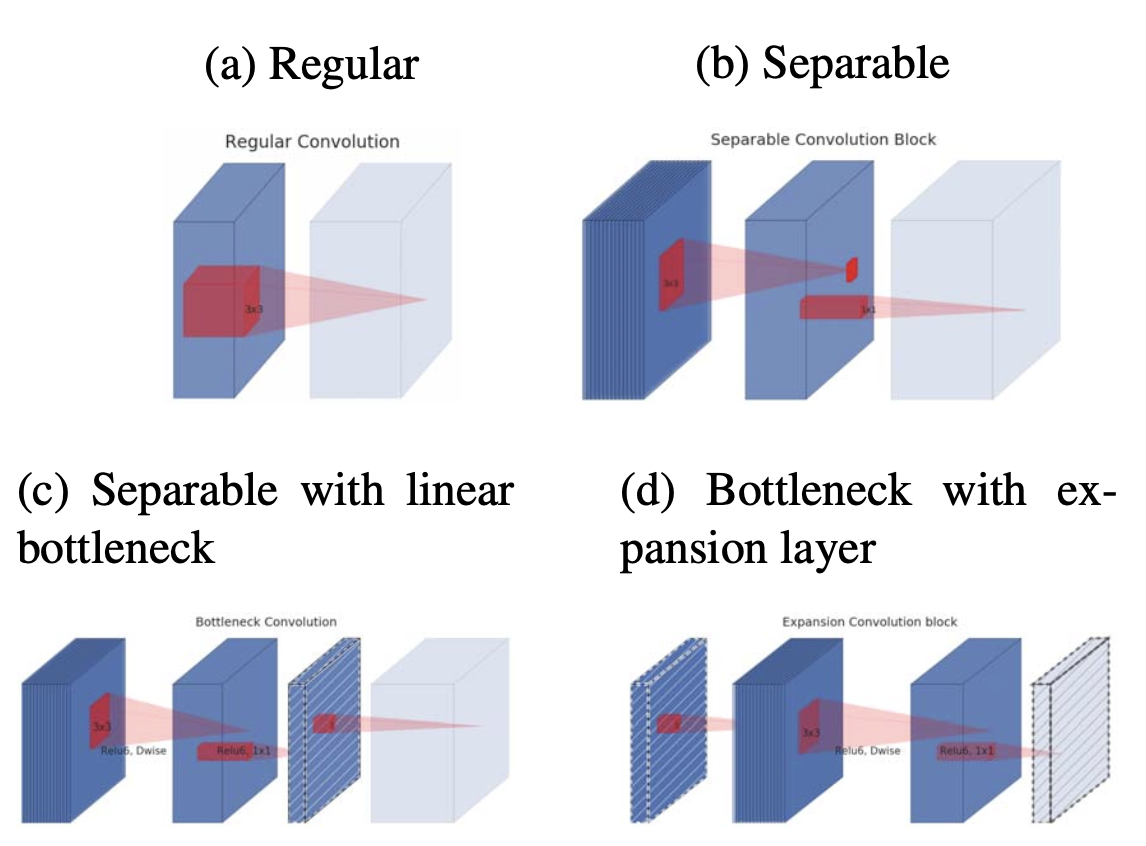
\includegraphics[width=0.8\textwidth]{images/figure7.png}
    \caption{The difference between residual block and inverted residual.}
    \label{fig:fig7}
  \end{figure}


\begin{figure}[H]
    \centering
    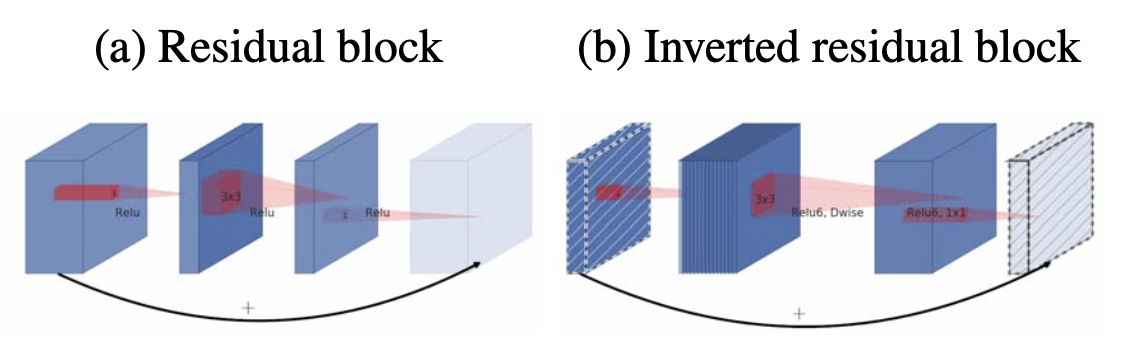
\includegraphics[width=0.8\textwidth]{images/figure8.png}
    \caption{Evolution of separable convolution blocks}
    \label{fig:fig8}
  \end{figure}
  
The structure of MobileNetV2 consists of 53 layers organized into 17 blocks, with a total of approximately 2.25 million parameters \cite{10.1109/ojemb.2021.3066097,10.1002/cpe.7405}. Each block employs a linear bottleneck design, which allows for the reduction of channels before applying depthwise convolutions and subsequently expanding them again through pointwise convolutions. This design minimizes the introduction of non-linearities that could hinder performance, thus enhancing the model's ability to learn complex features while remaining lightweight \cite{10.21203/rs.3.rs-4523549/v1,10.3389/fpls.2023.1321877}. The architecture also incorporates global average pooling at the end, converting the spatial input into a fixed-size vector suitable for classification tasks \cite{10.3389/fpls.2023.1321877,10.1109/cvpr.2018.00474}.


\begin{figure}[H]
    \centering
    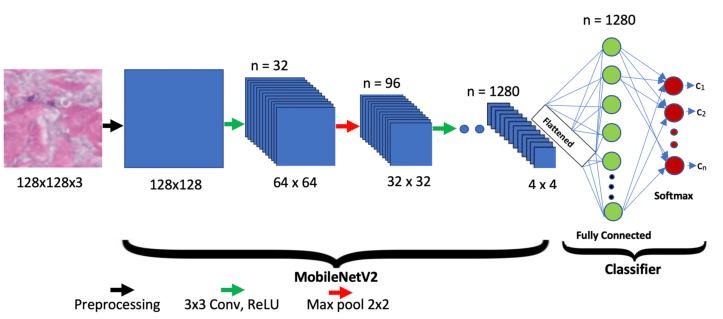
\includegraphics[width=0.8\textwidth]{images/figure6.png}
    \caption{MobileNetV2 network architecture \cite{10.1109/ojemb.2021.3066097}.}
    \label{fig:fig5}
  \end{figure}

MobileNetV2 has demonstrated remarkable versatility across various applications, including image classification, feature extraction, and real-time inference on devices with limited computational resources \cite{10.21203/rs.3.rs-4496133/v1,10.55927/mudima.v3i9.5924}. Its efficient design principles make it particularly well-suited for deployment in mobile applications, where speed and accuracy are critical \cite{10.55927/mudima.v3i9.5924,10.5109/6792818}. Furthermore, the architecture supports transfer learning, allowing it to leverage pre-trained weights for improved performance in specific tasks, even with smaller datasets \cite{10.1109/ojemb.2021.3066097,10.55927/mudima.v3i9.5924,10.14569/ijacsa.2023.01406105}.

\begin{figure}[H]
    \centering
    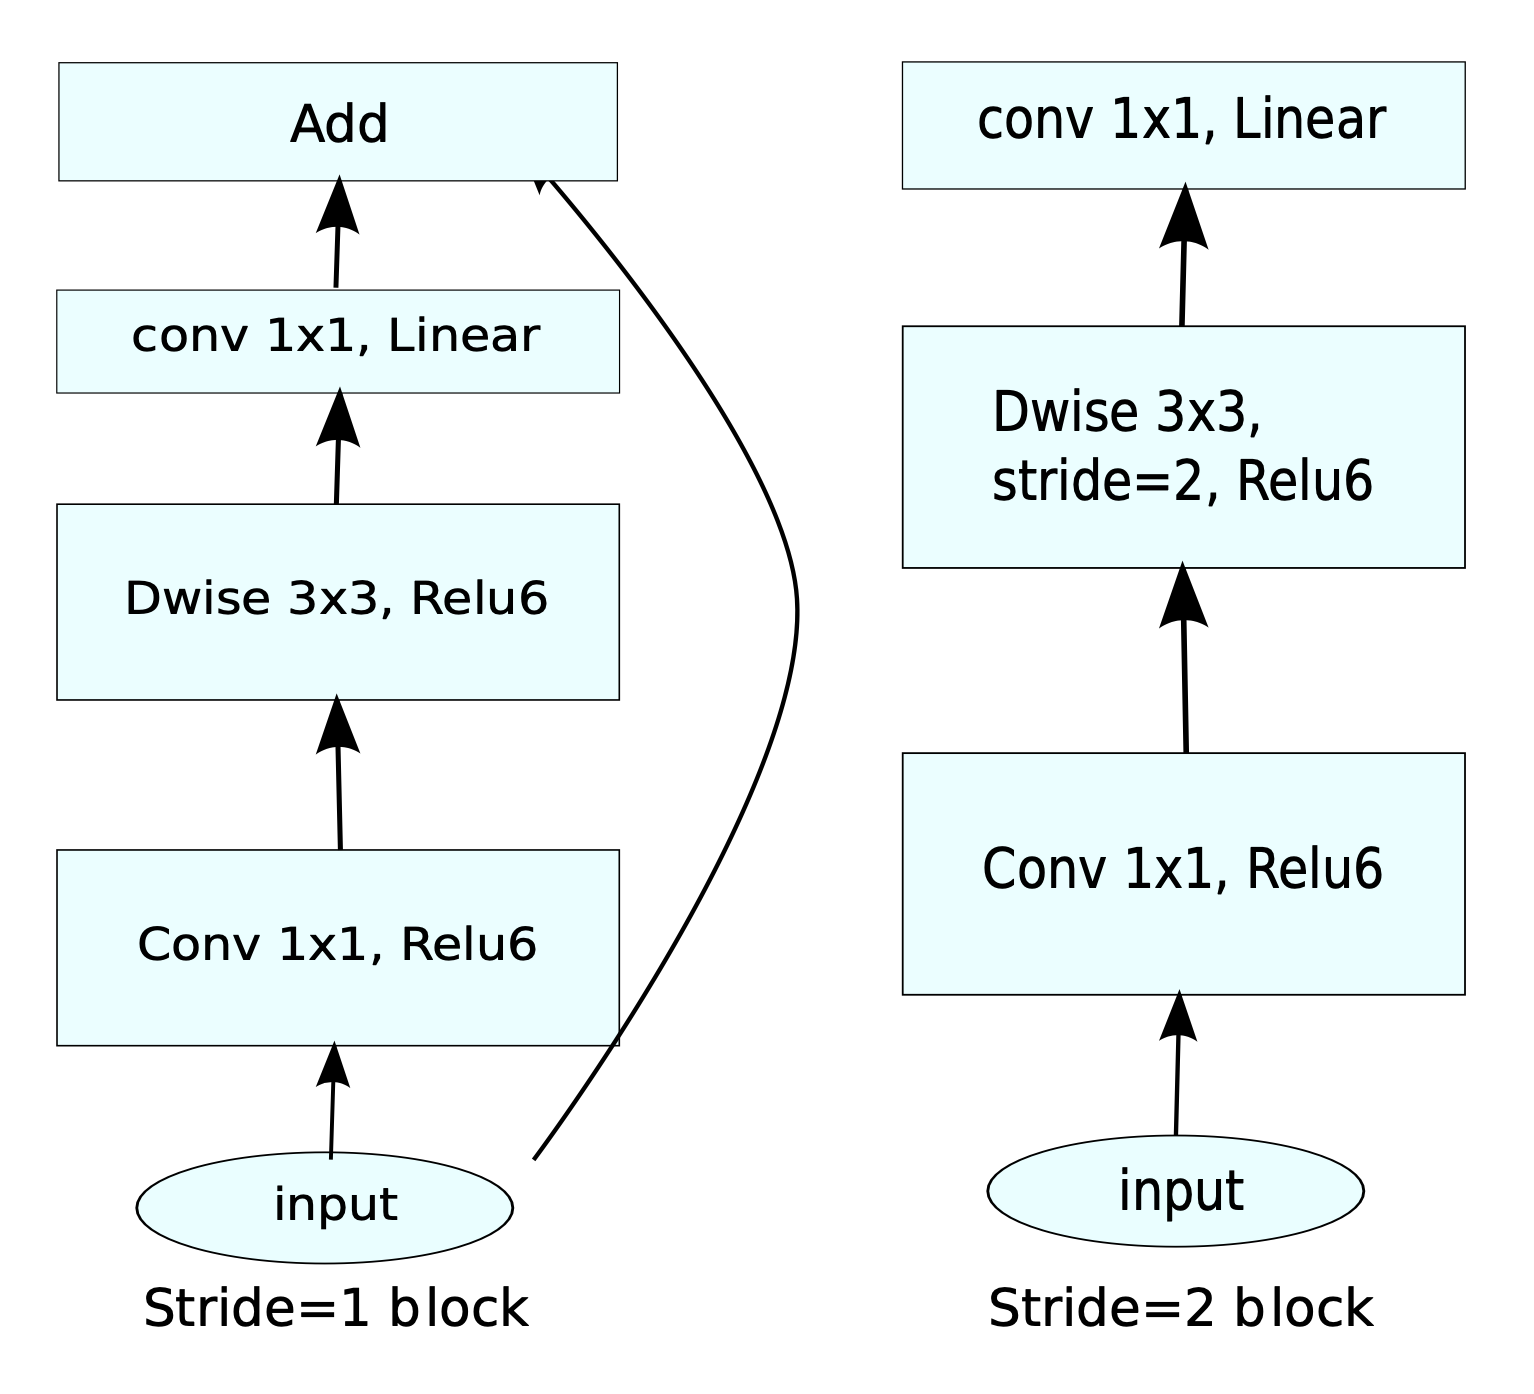
\includegraphics[width=0.8\textwidth]{images/figure5.png}
    \caption{MobileNetV2 layers.}
    \label{fig:fig6}
  \end{figure}

\subsection{Pretrained Model Selection}

The MobileNetV2 architecture was selected as the foundational model for traffic sign recognition due to its lightweight design and computational efficiency. MobileNetV2 is characterized by its use of depthwise separable convolutions and inverted residual structures, which significantly reduce the number of parameters and computational cost compared to standard convolutional networks \cite{10.1109/cvpr.2018.00474}. This architectural choice is particularly advantageous for mobile and edge devices, where computational resources are limited, allowing for efficient processing without sacrificing performance \cite{10.55927/mudima.v3i9.5924}. The lightweight nature of MobileNetV2 makes it highly optimized for real-time applications, which is crucial for deployment in vehicular environments where low-latency processing is essential \cite{10.55927/mudima.v3i9.5924}.

Moreover, initializing the model with pretrained weights on the ImageNet dataset allows MobileNetV2 to leverage rich feature representations, thereby expediting the convergence process during training \cite{10.1167/tvst.9.2.35}. This practice is supported by evidence that pretrained models can achieve better performance in various tasks, including image classification, by utilizing learned features from large datasets \cite{10.1167/tvst.9.2.35,10.48550/arxiv.1909.11229}. The effectiveness of this approach is further underscored by studies demonstrating that pretrained networks can enhance model robustness and generalization capabilities, particularly in scenarios with limited labeled data \cite{10.1101/2023.05.31.23290789}.

In summary, the selection of MobileNetV2 for traffic sign recognition is justified by its efficient architecture, suitability for real-time applications, and the benefits derived from transfer learning through pretrained weights on the ImageNet dataset.

\subsection{Dataset Partitioning}
The German Traffic Sign Recognition Benchmark (GTSRB) dataset was partitioned to facilitate effective training, validation, and testing. The training dataset was split using an 80/20 ratio, where 80\% of the data was allocated for training and 20\% for validation. This stratified partitioning ensures that the model generalizes well by validating its performance on unseen data during training. The test dataset was kept entirely separate to provide an unbiased assessment of the model's final performance.

\subsection{Image Preprocessing and Data Augmentation}
Robust image preprocessing and data augmentation techniques were applied to enhance the model's generalization capabilities. Training images underwent a series of transformations, including resizing to 224x224 pixels, random horizontal flipping, random rotations up to 15 degrees, and color jittering to simulate variations in lighting conditions. These transformations artificially increased the diversity of the dataset, mitigating overfitting. All images were subsequently converted to tensors and normalized using the ImageNet mean and standard deviation values to standardize the input distribution. Testing images were subjected to resizing and normalization only, ensuring consistent evaluation conditions.

\subsection{Fine-Tuning Strategy}
To adapt MobileNetV2 for traffic sign recognition, the final classification layer was replaced with a fully connected layer comprising 43 output nodes, corresponding to the number of traffic sign classes in the GTSRB dataset. All preceding convolutional layers were frozen to preserve the pretrained feature extraction capabilities, while the new classifier layer was fine-tuned to specialize in distinguishing between traffic sign categories. This selective fine-tuning strategy balances computational efficiency with task-specific learning.

\subsection{Training Configuration}

The model was trained over 10 epochs with a batch size of 16, utilizing the Adam optimizer with a learning rate of 0.001. Cross-entropy loss was employed as the objective function to handle the multi-class classification task. A validation split of 20\% within the training set enabled continuous performance monitoring and adjustment during training. These hyperparameters were chosen to provide an optimal trade-off between model convergence speed and generalization performance, ensuring efficient and stable learning across the dataset.

\section{VANET Simulation}

This VANET (Vehicular Ad-Hoc Network) simulation models how vehicles dynamically communicate with one another in a decentralized network. Each vehicle operates as a node capable of transmitting and receiving information within a specific communication range. This setup mirrors real-world vehicle-to-vehicle (V2V) communication used in intelligent transportation systems to improve traffic safety and efficiency.

\subsection{Network Interface Structure}
\begin{itemize}
    \item \textbf{Transmission:} Each vehicle is equipped with a \textit{Network Interface} that allows it to broadcast messages (such as alerts or detected hazards) to nearby vehicles. Transmission is limited by a \textit{communication range}, ensuring that only vehicles within proximity receive the information.
    \item \textbf{Reception Queue:} Vehicles maintain a \textit{reception queue} where incoming messages are stored. This queue ensures that vehicles can process multiple messages in an orderly fashion.
    \item \textbf{Processing Messages:} Vehicles periodically check their reception queue and act upon the received information, allowing them to adapt to traffic conditions or hazards.
    \item \textbf{Distance Calculation:} A key feature is the simulation of distance on a \textit{looped or circular road}, where the shortest path between vehicles is calculated, even if they are near the start and end of the road. This ensures continuous communication without boundary disruptions.
\end{itemize}

\subsection{Vehicle Initialization and Communication}
\begin{itemize}
    \item \textbf{Unique Vehicle IDs:} Each vehicle is assigned a unique identifier, distinguishing it within the network.
    \item \textbf{Vehicle Positioning:} Vehicles are placed at specific positions along a simulated road, which is critical for calculating communication ranges and message dissemination.
    \item \textbf{Dynamic Interaction:} As the simulation progresses, vehicles move and continually check for nearby vehicles to send or receive messages, simulating real-world traffic flow.
\end{itemize}

\subsection{Simulation Flow}
\begin{enumerate}
    \item Vehicles broadcast messages to nearby vehicles within their communication range.
    \item Vehicles receive and store incoming messages in their reception queue.
    \item Vehicles process messages to make decisions or pass the information along.
    \item The simulation repeats these steps over multiple iterations, reflecting continuous vehicle interaction.
\end{enumerate}

\subsection{Communication Efficiency}
\begin{itemize}
    \item The simulation evaluates how effectively vehicles can transmit and receive data in dynamic traffic conditions.
    \item By simulating road constraints (looped roads) and communication ranges, it models real-world challenges in VANET systems.
\end{itemize}

\section{Simulating Adverse Conditions}

The primary goal of training the model and developing the VANET simulation system was to evaluate its performance under various conditions and assess its resilience.

For each condition, two sets of tests were conducted:

\begin{enumerate}
    \item \textbf{Independent Vehicle Test:} A single vehicle operated without any connection or communication with other vehicles, relying solely on its own recognition capabilities.
    
    \item \textbf{VANET System Test:} The same conditions were applied, but this time vehicles communicated and shared information. Predictions were made collaboratively through a consensus mechanism, allowing vehicles to collectively interpret traffic signs.
\end{enumerate}

The environmental conditions used for testing were:

\begin{enumerate}
    \item Normal (no alterations)
    \item Brightness variation
    \item Motion blur
    \item Angle and rotation adjustments
\end{enumerate}

\subsection{Normal (no alterations)}

To initiate the tests and simulations, both the system and the standalone vehicle were evaluated using the original dataset
 without any modifications or simulated conditions. This was a standard test conducted on the dataset's test set. Regardless
  of being part of the VANET system or operating independently, all vehicles utilized the same model to generate predictions
   on the identical dataset.

\subsection{Brightness Variation}

Considering that vehicles are equipped with headlights of varying intensities, producing different levels 
of brightness and illuminating varying distances ahead, we assumed that this could lead to differences in 
recognition performance. Each vehicle, having a unique set of headlights, may perceive and interpret its 
surroundings differently under such conditions. 

Additionally, environmental lighting plays a significant role, as vehicles may be positioned at varying distances 
from streetlights, resulting in different visibility conditions for each vehicle.

\begin{figure}[H]
    \centering
    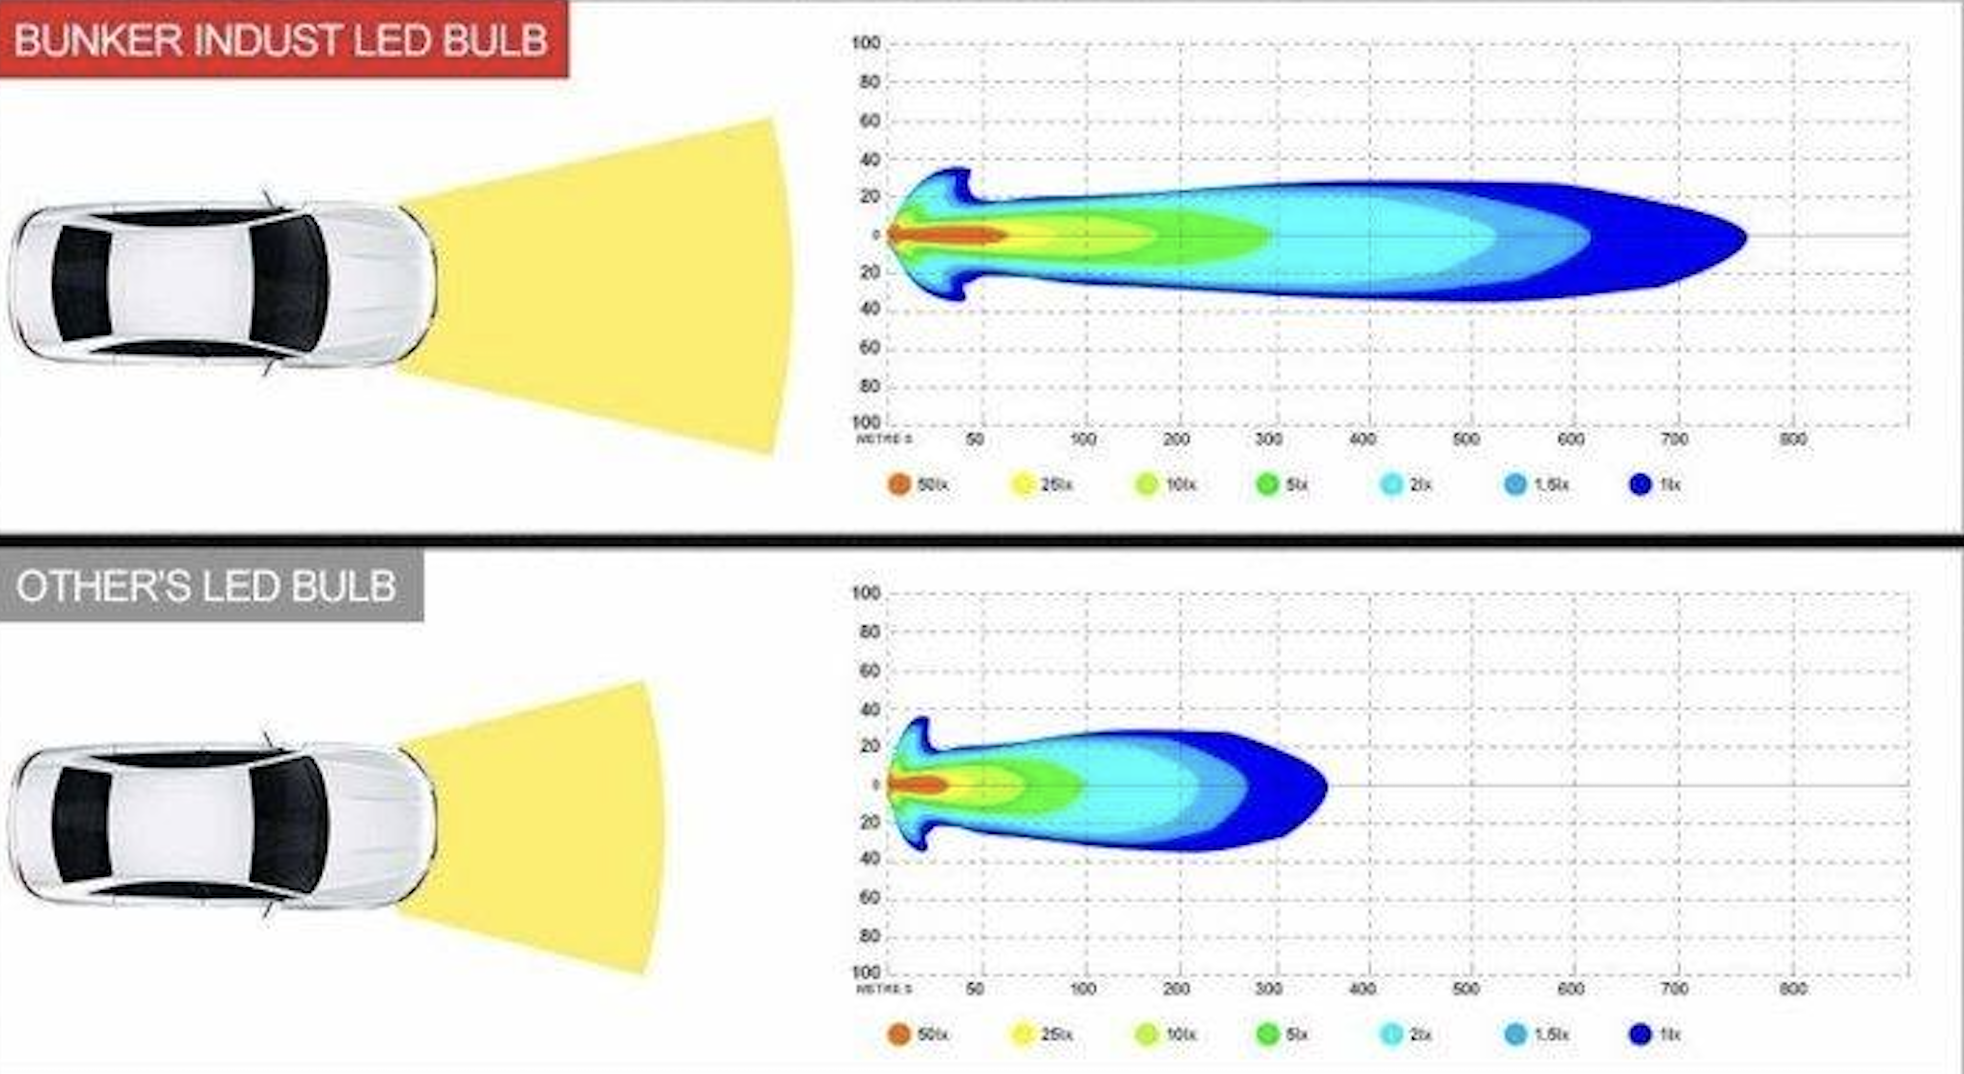
\includegraphics[width=0.8\textwidth]{images/figure10.png}
    \caption{Different luminosity and light coverage on different vehicles.}
    \label{fig:fig9}
  \end{figure}

  \subsubsection{Adjustment}

  explain how the heck you did that. 
  randomness and the image processing side of it. 

\subsection{Motion Blur}

\subsection{Angle and Rotation Adjustments}





